%\chapter{Su Memoria}

La Real Armada Española \index{armada!española} honra la memoria de
Blas de Lezo \index{Blas de Lezo}con el mayor honor que puede
rendirse a un marino español: tiene por costumbre inveterada que uno
de sus buques lleve su nombre. El último así bautizado es una fragata
de la clase Álvaro de Bazán: la Blas de Lezo (F-103). Anteriormente
portaron dicho nombre un cañonero de la clase Elcano, llamado General
Lezo, que en 1898 se encontraba en Filipinas, aunque no llegó a
participar en los combates al tener las calderas desmontadas, el
crucero Blas de Lezo, que se perdió en 1932 al tocar un bajío frente a
las costas de Finisterre y un destructor procedente de la ayuda
estadounidense, el Blas de Lezo (D-65). La Armada Colombiana
\index{armada!colombiana} también tuvo un buque con el nombre del
almirante, el ARC Blas de Lezo (BT-62), un petrolero de clase
Mettawee, adquirido a la Armada de los Estados Unidos \index{armada !
  de EEUU} el 26 de noviembre de 1947 y dado de baja en enero de 1965.

\begin{figure}[!hbp]
\centering
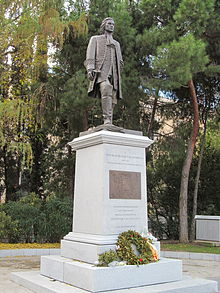
\includegraphics[width=.35\textwidth]{jpg_Blas_de_Lezo_00.jpg}
\caption{\label{fig:donBlas01} Estatua en honor del teniente general
  de la Armada Blas de Lezo en la plaza de Colón en Madrid realizada
  por Salvador Amaya.}
\end{figure}

El 12 de marzo de 2014 se inauguró en el Paseo de Canalejas de la
ciudad de Cádiz el primer monumento dedicado a Blas de Lezo en
España. Al acto acudieron el embajador de Colombia en España y un
almirante de la Armada Española.\index{armada!española} En la
fachada de la Diputación Foral de Guipúzcoa, situada en San Sebastián,
se encuentra desde 1885 un busto de Blas de Lezo, oriundo de Pasajes.

El 15 de noviembre de 2014 el rey Juan Carlos inauguró en los jardines
del Descubrimiento de la plaza de Colón de Madrid una escultura en
bronce de 3,5 metros ---7 metros en total contando con el pedestal---
con la efigie del almirante, muy próxima a la de otros dos marinos
ilustres de la Armada Española como fueron Cristóbal Colón y Jorge
Juan y Santacilia. El monumento fue sufragado íntegramente por
suscripción popular con las aportaciones que un millar de ciudadanos
de todos los rincones de España hicieron a la Asociación Monumento a
Blas de Lezo. \index{Blas de Lezo} Cuatro días después el Ayuntamiento
de Barcelona aprobó una moción con los votos de CiU, ICV, ERC y DCst,
y con la abstención del PSC, en la que se pedía al Ayuntamiento de
Madrid que retirara la estatua por haber participado Blas de Lezo en
el bombardeo de Barcelona durante la Guerra de Sucesión Española. La
petición fue rechazada en rueda de prensa por el ayuntamiento de la
capital.

Existe una placa en su honor en el Panteón de Marinos Ilustres en San
Fernando (Cádiz), donde reposan otros héroes de la Armada
Española. \index{armada!española} También existe una maqueta de la
batalla de Cartagena de Indias \index{Cartagena!de Indias} en la
Academia de Ingenieros de Hoyo de Manzanares (Madrid). Análogamente,
en el Museo Naval de Cartagena de Indias se exhibe un conjunto de
maquetas con detalle de las fortificaciones de aquella bahía y que
describen el sitio de la ciudad por el almirante Vernon, la defensa
organizada por Don Blas de Lezo, \index{Blas de Lezo} y su victoria
sobre el inglés.

Existen calles con su nombre en las ciudades de Valencia, Málaga,
Alicante, Cartagena de Indias, Las Palmas de Gran Canaria, San
Sebastián, Cádiz, Huelva, Fuengirola, Rentería, Irún, Pasajes ---su
localidad natal, y finalmente, tras una recogida de firmas, el 28
de abril de 2010 se aprobó dedicarle una avenida en la capital de
España, Madrid.

Sin embargo, aunque las proezas de Blas de Lezo \index{Blas de Lezo}
están a la altura de los más grandes marinos de la historia, es un
personaje histórico no suficientemente reconocido, ni su biografía
merecidamente divulgada.133 Por esa razón, la empresa española
DL-Multimedia está preparando un documental sobre su vida para los
canales Historia y Odisea.

Blas de Lezo \index{Blas de Lezo} es, al contrario, un reconocido
héroe en Cartagena de Indias, que le rinde homenaje de varias maneras:
barrios, avenidas y plazas le conmemoran en sus nombres; y su estatua
frente al castillo San Felipe de Barajas mantiene vivo entre los
cartageneros el recuerdo del defensor de su ciudad. El 5 de noviembre
de 2009, en Cartagena de Indias, se dio cumplimiento a un deseo de
Blas de Lezo, que en su testamento pedía que un grupo de españoles
pusiese una placa que conmemorase aquella victoria. En la inscripción
se puede leer:

\begin{displayquote}
  Homenaje al Almirante D. Blas de Lezo y Olavarrieta. Esta placa se
  colocó para homenajear al invicto almirante que con su ingenio,
  valor y tenacidad dirigió la defensa de Cartegena de Indias. Derrotó
  aquí, frente a estas mismas murallas, a una armada británica
  \index{armada!británica} de 186 barcos y 23.600 hombres, más 4000
  reclutas de Virginia. Armada aún más grande que la Invencible
  Española que los británicos habían enviado al mando del Almirante
  Vernon para conquistar la ciudad llave y así imponer el idioma
  inglés en toda la América entonces española. Cumplimos hoy juntos,
  españoles y colombianos, con la última voluntad del Almirante, que
  quiso que se colocara una placa en las murallas de Cartagena de
  Indias que dijera: Aquí España derrotó a Inglaterra y sus
  colonias. Cartagena de Indias, marzo de 1741.
\end{displayquote}

Asimismo, el 21 de noviembre de 2009 se descubrió para su memoria una
placa en la calle Larga nº 70 del Puerto de Santa María, ciudad donde
residió Blas de Lezo antes de librar la batalla de Cartagena y donde
nacieron algunos de sus hijos. En dicho acto se estrenó la marcha
militar Almirante Blas de Lezo, compuesta para la Real Armada por
Joaquín Drake García, e interpretada por la Banda de Música del Tercio
Sur (Infantería de Marina). Presidieron el acto el Almirante de la
Flota, el Alcalde de la ciudad y la presidente del Club de Mar Puerto
Sherry. La lápida reza: «En 1736 vivió en este lugar junto a su
familia el Teniente General de la Armada D. Blas de Lezo y
Olavarrieta, insigne e invencible marino, héroe de la Batalla de
Cartagena de Indias en la que la flota inglesa sufrió una humillante
derrota en el año 1741. La ciudad del Puerto de Santa María en
homenaje a su memoria. 21 de noviembre de 2009».
